\section{Camera Theory}
An image captured through a camera is the result of reflected light being detected on a camera sensor, see figure \ref{fig:light_cam}. This process is know as \textit{image acquisition} and is generally not something you think about when you capture an image with a camera, since it all happens automatically. In this chapter the basics of image acquisition using a digital camera will be explained. To understand how this works it is necessary to have a basic understanding of the physics behind light.

\begin{figure}[htbp] 
\centering 
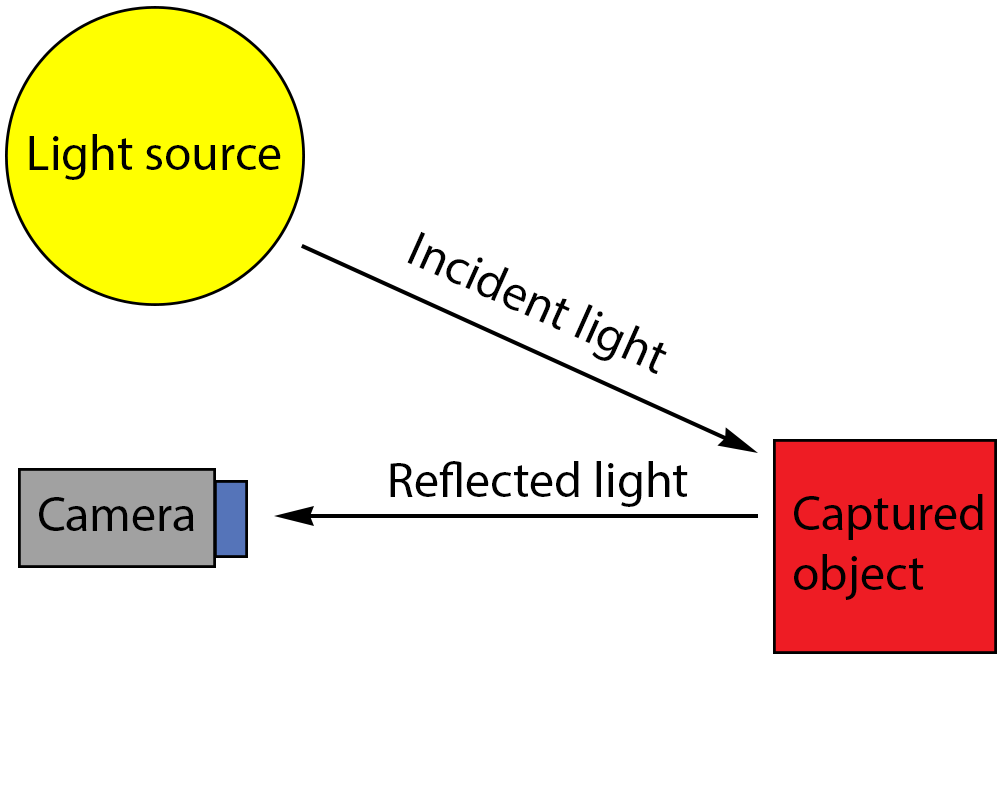
\includegraphics[width=0.5\textwidth]{Pictures/Theory/light_from_sun.png} 
\caption{Light as captured by a camera} 
\label{fig:light_cam} 
\end{figure}

Light is a form of electromagnetic radiation and can be viewed as both waves and particles. This duality is however not something that will be concerned within this chapter; the wave model is sufficient to build the foundation of the understanding we need. A light wave is a small packet of energy traveling through space. These energy packets are known as photons. Photons can be described by three properties:

\begin{itemize}
\item \textbf{Wavelenght} - Measured in meters from wave top to wave top and denoted as $\lambda$.
\item \textbf{Frequency} - Measured in oscillations per second, Hz, denoted $f$.
\item \textbf{Energy} - Measured in electronvolts, eV, denoted $E$.
\end{itemize}

The formulae for these properties are as follows:
To derive the wavelength or the frequency, formula \ref{eq:wavelenght} is applied:
\begin{align}
\centering 
\lambda = \frac{C}{f}
\label{eq:wavelenght} 
\end{align}
$\lambda$ and f we are familiar with, and C is the speed of light. The second equation, equation \ref{eq:e_v}, describes the energy:
\begin{align}
\centering
E = \frac{hC}{\lambda}
\label{eq:e_v} 
\end{align}
where h is Planck's constant, which describes the proportional relationship between energy of a photon and an the corresponding electromagnetic wave's frequency. E, C and $\lambda$ are still as explained above.

The wavelength of the photon determines what color one perceives. However; as we know from physics, the speed of light is constant; thus changing the frequency will alter the wavelength and therefore the color that is perceived. The visible spectrum of light is but a fraction of the full spectrum of electromagnetic radiation \fixme{SEE THE FIGURE THAT IS NOT THERE}. As with images, light interacts additively, with a mix of equal parts of each wavelength resulting in white light.
\fixme{image of light color by wavelength}
The most common light source by far is the sun. The white light from the sun can be broken down into its component wavelengths by refracting the light in a prism. This will yield the full color spectrum\fixme{MORE PICTURES; LIGHT REFRACTED}.
While different wavelengths correspond to different colors, these colors only remain defined within our perception. The reason we see ~600nm light as yellow is because our eyes contain three types of optically sensitive cells, known as \textit{cones}, constructed to be sensitive to three colors; red, green and blue. 600 nm lies between the green and red cells, thus both cells are firing and the perceived color becomes yellow.\citep{perception_book}.\fixme{link to cells and visible spectrum maybe figures?}
\subsection{Digital image acquisition}
When capturing an image using a digital camera, light is passed through a lens onto the sensor, which acts in much the same way as our eyes. In place of cones sensitive to specific wavelengths, a camera sensor has a physical matrix of pixel sensors, one for each pixel in the output image. A camera that can only capture black and white photos have only one type of sensor in each physical pixel whereas a camera that captures RGB color images has three types of sensors in each pixel. \fixme{sources and images?}
\subsection{Image acquisition in the project}
In the project, two cameras were contemplated; a normal RGB webcam and a similar camera with an infrared (IR) filter installed. The filter consists of a small strip of normal analogue film, used for analogue pictures, that has been mounted on the lens. The film strip allows only infrared light to pass, thus making the only light that reaches the sensor infrared. 

\begin{figure}[htbp] 
\centering 
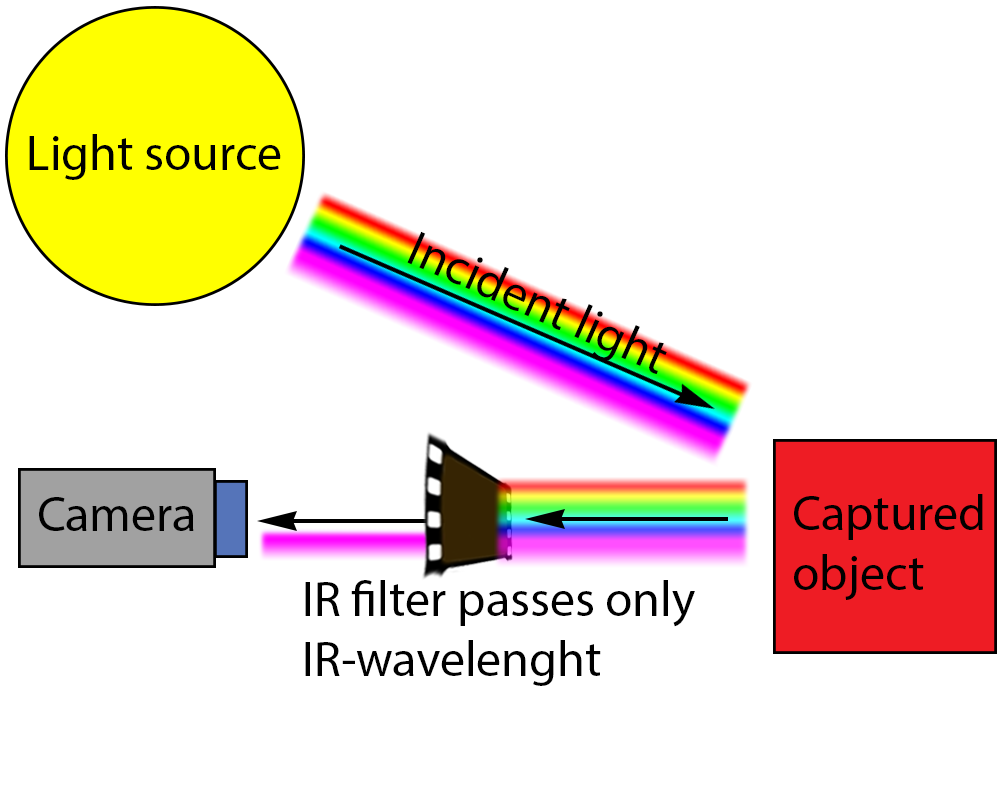
\includegraphics[width=0.5\textwidth]{Pictures/Theory/IR_filter.png} 
\caption{The IR filter only allows infrared ligh to pass} 
\label{fig:ir_filter} 
\end{figure}

This is interesting, as it enables a larger degree of control over the illumination in the scene that is captured. Normally in a scene, controlling the lighting  \fixme{should be refenrence to place where we state that light is hard to control and the issues inherit in handling lighting "on location"} can prove a challenge, and in order to operate without error an image processing algorithm would have to take into account the variance in lighting that occurs naturally during a day cycle. Working with IR eliminates this issue.